\documentclass[logo,reportComp]{thesis}
\usepackage[cpp,pseudo]{mypackage}

\title{高级编程技术实验报告}
\subtitle{实验一:空间奶牛传输}
\school{数据科学与计算机学院}
\author{陈鸿峥}
\classname{17大数据与人工智能}
\stunum{17341015}
\headercontext{高级编程技术实验报告}
% \authorremark{本实验报告用\LaTeX撰写,创建时间:\builddate\today}
\lstset{language=python}

\begin{document}

\maketitle

\section{问题描述及求解思路}

\subsection{Part A: Transporting Cows Across Space}
\subsubsection{读入数据}
先创建一个空字典,然后利用python的\verb'with...as...'语句读入文件,有效避免文件不存在或忘记关闭等情况(会自动报错)。

然后直接枚举文件的每一行,通过\verb'split'对字符串进行分割,存在二元组里,进而创建字典项。
\begin{lstlisting}
res = {} # create an empty dictionary
with open(filename,"r") as file: # avoid exception
    for line in file:
        (name,num) = line.split(',')
        res[name] = int(num) # remember to take int
\end{lstlisting}

\subsubsection{贪心算法}
先对读入的字典按照value进行降序排列,利用python的\verb'sorted'函数可以很方便做到。
同时\verb'sorted'会返回一个新的列表,避免对原字典的破坏。
这里还利用了\textbf{lambda表达式},指明是以value为key排序。
\begin{lstlisting}
cow_sorted = sorted(cows.items(),key=lambda item:item[1],reverse=True)
\end{lstlisting}

然后每次遍历\verb'cow_sorted',从大到小依次添加不会超过\verb'limit'的表项,每添加一项就从列表中删除该项。
每执行完一次遍历,就将当前\verb'trip'添加到结果数组\verb'res'中。
然后重新开始新一轮遍历,直到\verb'cow_sorted'为空。
代码如下,已将原题注释删除。
\begin{lstlisting}
def greedy_cow_transport(cows,limit=10):
    # Firstly sort the dict by value
    # The code below will not ruin the original dict
    cow_sorted = sorted(cows.items(),key=lambda item:item[1],reverse=True)
    res = []
    # the input must ensure the biggest cow <= limit
    while (len(cow_sorted) > 0):
        curr_weight = 0
        one_trip = []
        for item in cow_sorted[:]: # copy out!
            if (curr_weight + item[1] <= limit):
                curr_weight += item[1]
                one_trip.append(item[0]) # append the name
                cow_sorted.remove(item)
        res.append(one_trip) # add the last
    return res
\end{lstlisting}

\subsubsection{暴力算法}
暴力算法十分直接,就是枚举每一个\verb'partition',判断该\verb'partition'是否合法,即\verb'partition'中每一个\verb'trip'的总重不超过\verb'limit'。
如果不合法,直接跳到下一个\verb'partition';合法,则判断是否为当前轮数最少,如果是,则更新最小轮数。
代码如下,已将原题注释删除。
\begin{lstlisting}
def brute_force_cow_transport(cows,limit=10):
    lst = cows.items() # will not ruin the original dict
    min_num_trip = len(cows)
    min_trip = []
    for partition in get_partitions(lst):
        flag = False # use for test if all trips valid
        for trip in partition:
            weights = sum([item[1] for item in trip]) # sum all weights in one trip
            if (weights > limit):
                flag = True
                break
        if flag:
            continue
        elif (len(partition) < min_num_trip): # find the min trip
            min_num_trip = len(partition)
            min_trip = [[item[0] for item in trip] for trip in partition] # take out all the names
    return min_trip
\end{lstlisting}

\subsubsection{比较时长}
将两种方法分别放在两个\verb'time.time()'中即可测定运行时间。
代码见\verb'ps1a.py',运行结果见图\ref{fig:a}。

\subsubsection{分析}
本部分为Problem A.5:Writeup的内容。
\begin{enumerate}
	\item 结果见图\ref{fig:a},除了一组原始测试样例外,还给出了自己的测试样例。
	从图\ref{fig:a}中可以看出,贪心算法明显比暴力算法快几个数量级。
	因为贪心算法只需对原字典进行一次排序,然后从大到小依次遍历插入即可,而且插入的项在原表项中可以直接删除,越到后面遍历的元素越少,最坏情况下也是平方级时间复杂度。
	而暴力算法的瓶颈在于划分\verb'get_partitions',需要将所有可能的排列划分全部枚举出来,这是指数级时间复杂度。
	故明显贪心比暴力要快。
	\item 贪心算法不一定能返回最优解,因为它之关心当前轮次是否有办法尽可能多地运满,而不考虑之后地轮次,故这是一种鼠目寸光,只在乎眼前的策略,好的情况可以达到最优解(如我给的测试样例),但坏的情况就不行了(如原题测试样例)。
	\item 暴力算法一定能返回最优解,因为它相当于枚举了所有可能的情况,然后从中挑选出一个最好的,这当然是全局最优解。
\end{enumerate}


\subsection{Part B: Dynamic Programming: Hatching a Plan}
\subsubsection{动态规划}
本题为典型的背包问题,对于每一个目标重量,枚举所有可能的鸡蛋重量(由于有无限鸡蛋),然后判断是否应该将该鸡蛋放入,放入总数量加1,不放则不做处理。

对于某一个目标重量$w_t$,其最优的鸡蛋数目$f(w_t)$满足下列动态转移方程
\[f(w_t)=\begin{cases}0 & w_t=1\\\min\{1+f(w_t-w_e)\},\forall w_e & w_t\geq 1\end{cases}\]
其中$w_e$为每一个鸡蛋的重量。

进而可以使用bottom-up的方法,对不同$f(w_t)$进行计算,最终得到$f(target_weight)$。
代码如下,原题注释已删减。
\begin{lstlisting}
def dp_make_weight(egg_weights, target_weight, memo = {}):
    memo[0] = 0
    for target in range(1,target_weight+1):
        for weight in egg_weights:
            if (target >= weight):
                # DP transition equation
                memo[target] = min(memo.get(target,target),1+memo[target-weight])
    return memo[target_weight]
\end{lstlisting}

\subsubsection{分析}
本部分为Problem B.2:Writeup的内容。
\begin{enumerate}
	\item 注意这是一个无限背包问题,这相当于解下面的不定方程
	\[w_1x_1+w_2x_2+\cdots+w_{30}x_{30}=W,\;x_i\geq 0,i\in\{1,2,\ldots,30\}\]
	其中$w_i$为每个鸡蛋的重量,$W$为目标重量,$x_i$为要求解的每个鸡蛋的数目。
	由于每个$x_i$都是非负数,故要进行暴力枚举,最差的情况要进行$(W+1)^{30}$种排列组合\footnote{这只是一个粗略估计,并未考虑$w_i$的顺序、大小等问题},这个数字太过庞大,显然是不可能实现的。
	\item 最开始我就采用了如下的贪心算法,但后来我发现并不能求到最优解。
\begin{lstlisting}
if (len(egg_weights) == 0):
    return 0
num_eggs = target_weight // egg_weights[-1]
return num_eggs + dp_make_weight(egg_weights[:-1],target_weight-num_eggs*egg_weights[-1])
\end{lstlisting}
	目标函数即为
	\[f(w_t)=w_t\opdiv w_e+f(w_t-w_e*(w_t\opdiv w_e))\]
	其中$w_e$已经按照降序排列,边界情况见程序。
	限制条件即鸡蛋是否已经由大到小被挑选完。
	策略同目标函数,每次选择最重鸡蛋,然后尽可能多地用最重填,填不满的部分再用轻的鸡蛋。
	\item 不一定,如图\ref{fig:b}中给的第二个测试样例。
	鸡蛋重量分别为$(1,5,11)$,目标重量为$15$。
	如果用贪心算法,先选$1$个$11$,剩下$4$没得选,只好填$4$个$1$,共$5$个鸡蛋。
	但采用动态规划,可以求得只用$3$个$5$单位重量的鸡蛋。
\end{enumerate}

\section{代码}
代码实施及注释请见附件\verb'ps1a.py'、\verb'ps1b.py'。

\section{运行截图}
实验运行结果如下面几幅图片所示,\textbf{注意给出了多个自己写的测试样例,确保结果的正确性和鲁棒性}。
\begin{figure}[H]
\centering
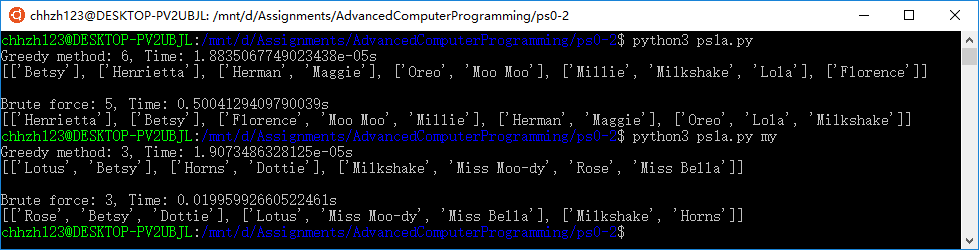
\includegraphics[width=\linewidth]{fig/a.PNG}
\caption{Part A结果,给出测试样例和自己写的样例输出}
\label{fig:a}
\end{figure}

\begin{figure}[H]
\centering
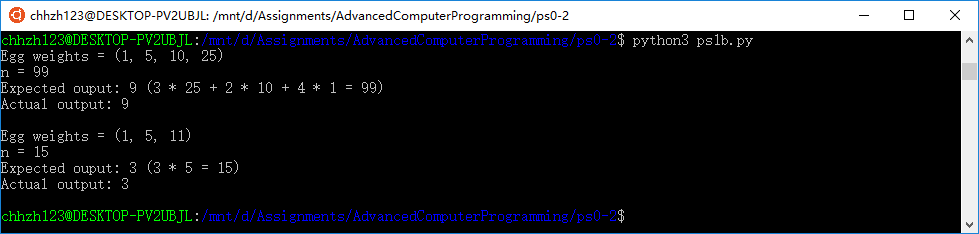
\includegraphics[width=\linewidth]{fig/b.PNG}
\caption{Part B结果,给出测试样例和自己写的样例输出}
\label{fig:b}
\end{figure}

\end{document}

% 实验提交内容
% 邮件主题,作业文件命名规范(学号、姓名)
% 文档pdf格式(问题、求解思路、代码、注释、运行截图)
% 考虑健壮性、可读性
% 极端样例